\documentclass[twocolumn]{article}

\usepackage{amsmath,amssymb,amsfonts}
\usepackage{xcolor}
\usepackage{listings}
\usepackage{inputenc}
\usepackage{graphicx}
\usepackage{authblk}

\providecommand{\keywords}[1]
{
  \small	
  \textbf{\textit{Keywords---}} #1
}

\begin{document}
\author[1]{Eric Raphael Huiza Pereyra}
\affil[1]{Department of Postgraduate Studies, Pontifical Catholic University of Peru}
\affil[]{\textit{eric.huiza@pucp.edu.pe}}

\title{\vspace{-2.0cm}\textbf{Method to detect gestures in a poorly annotated dataset}}

\maketitle
    
\begin{abstract}
Include abstract here \\
\keywords{video classification,gestures detection}
\end{abstract}

\section{Introduction}

The World Health Organization (WHO) stated that 466 million people world wide have disabling hearing loss and it is estimated that by 2050 over 900 million people will have disabling hearing loss and represents a global cost of 750.00 million dollars annually  \cite{deafness_and_hearing_loss_2019}. 

The Peruvian Institute of Informatics and Statistics (INEI) executed a national disabilities survey with the objective to better understand which disabilities affect the Peruvian population  

En el Perú, según la última encuesta nacional especializada por discapacidad del instituto peruano de Estadística e Informática INEI realizada durante el año 2012 y publicada en marzo del 2014, el 1.8\% de la población presenta limitaciones auditivas permanentes.

El día de hoy ya es completamente viable pensar en sistemas que puedan detectar y transcribir lenguajes de señas. Sin embargo los lenguajes de señas varían mucho en diferentes regiones, y es muy costoso preparar un corpus que permita entrenar los modelos de inteligencia artificial. El Grupo de Investigación de Señas Gramaticales de la Pontificia Universidad Católica del Perú (PUCP) ha hecho el esfuerzo de crear este corpus para el Lenguaje de Señas Peruano (LSP), el cual está débilmente anotado, es decir, no se tiene anotado de manera exacta el instante en que se emite una seña y su traducción.

Este estudio se ha realizado para la obtención del grado de Magister en Informática con mención en Ciencias de la Computación durante el periodo 2019 y trata de responder las siguientes preguntas:
\begin{itemize}
\item ¿Cuales son las técnicas disponibles más relevantes para el entrenamiento de un modelo de aprendizaje de máquina a partir de contenido visual y transcripción de audio y video débilmente anotado?
\item ¿Qué tan preciso y exhaustivo es el modelo descrito en la pregunta anterior en el reconocimiento de un conjunto reducido de señas a partir de un conjunto de datos débilmente anotado?
\item ¿Cual es la relación entre el número de muestras y la detección de nuevos elementos del Lenguaje de Señas Peruano en cuanto al rendimiento en cuanto a precisión y exhaustividad del método?
\end{itemize}
contribuyendo en el desarrollo de un método generalizable para la detección progresiva de señas que hará uso del corpus del LSP elaborado por la PUCP. Asimismo los resultados del estudio servirán como base a futuras investigaciones como la mejora de la accesibilidad a sistemas informáticos y la interacción humano computador para personas con discapacidades auditivas o de habla.
\section{Related Work}
\section{Method}
\section{Experimentation}
\subsection{Dataset Description}
Este estudio hace uso del corpus de la LSP elaborado por el Grupo de Investigación en Señas Gramaticales de la PUCP el cual está limitado a 24 informantes, 12 hombres y 12 mujeres, todos residentes en Lima. Todos reportaron ser sordos de nacimiento o de manera pre-locutiva, es decir, antes de la adquisición del Castellano. El corpus esta conformado por total de 718 clips de video traducidos al Castellano, los cuales se encuentran disponibles en el Archivo Digital de Lenguas Peruanas de la PUCP (http://repositorio.pucp.edu.pe/index/handle/123456789/15344)

El corpus se encuentra débilmente anotado ya que no existe una relación directa entre la traducción y el momento en que se emite la seña.

\subsection{Video Annotation}
\begin{figure}[ht!]
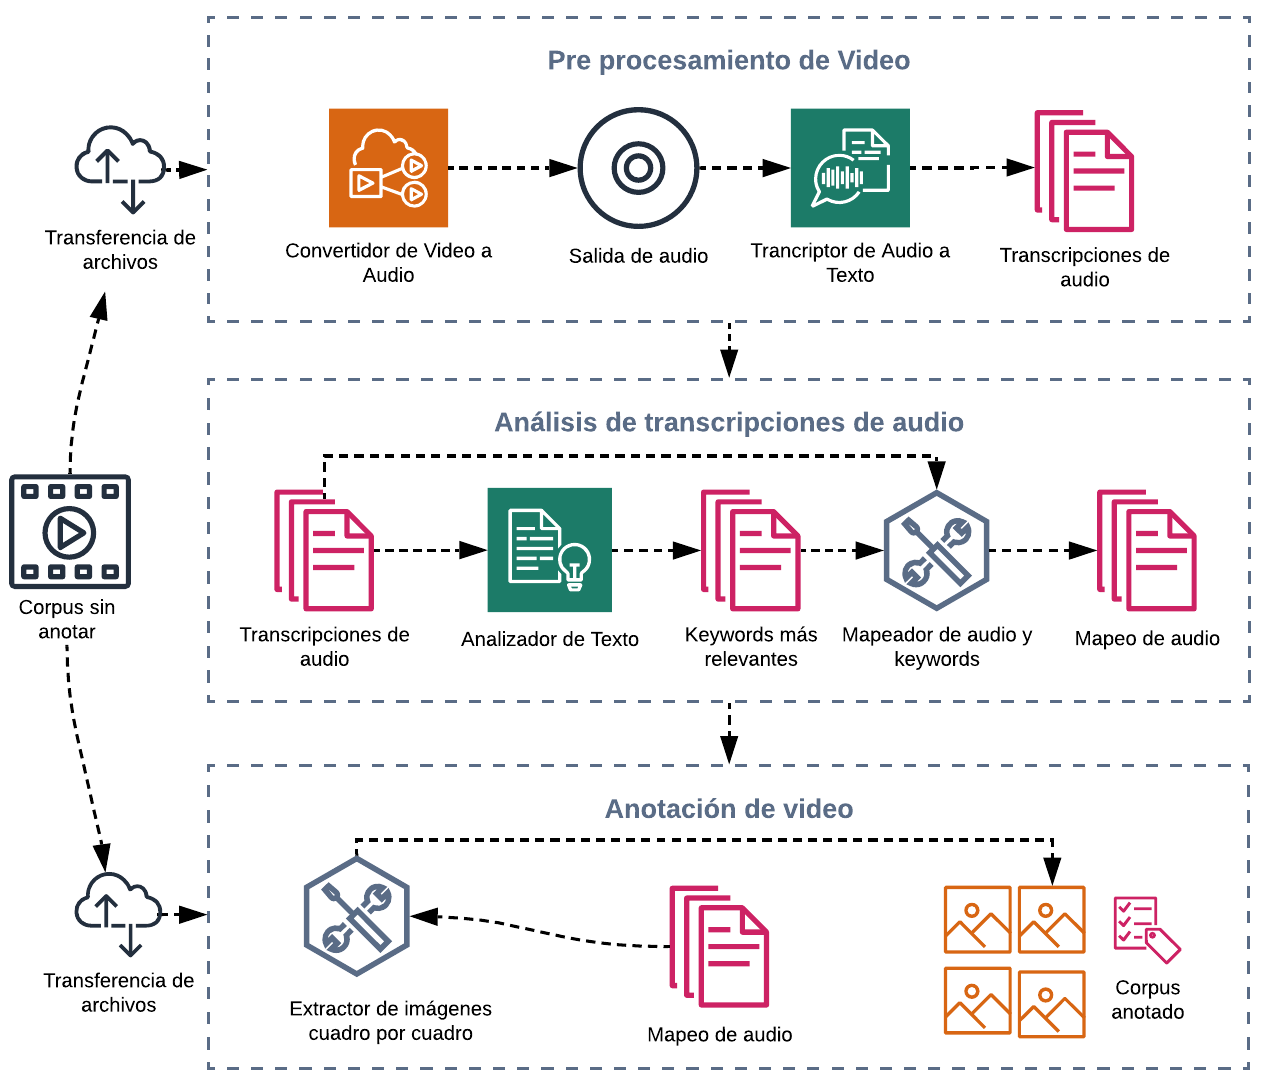
\includegraphics[width=\linewidth]{video-annotation-pipeline.png}
\caption{Video annotation process}
\end{figure}
\section{Conclusion}

\bibliographystyle{ieeetr}
\bibliography{References}


\end{document}
